\documentclass[tikz,border=3.14mm]{standalone}
\usepackage{tikz}
\usetikzlibrary{calc,patterns,angles,quotes}

\begin{document}

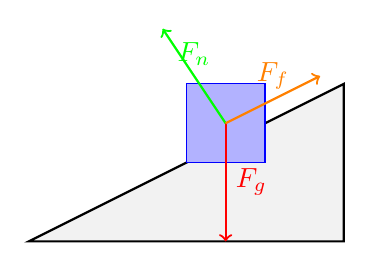
\begin{tikzpicture}
    % Draw the inclined plane
    \draw[thick,black,fill=gray!10] (0,0) -- (4,2) -- (4,0) -- cycle;

    % Place the block
    \draw[blue,fill=blue!30] (2,1) rectangle ++(1,1);

    % Draw the forces
    % Force of gravity
    \draw[red,thick,->] ($(2,1)+(0.5,0.5)$) -- ++(0,-1.5) node[midway,right] {$F_g$};
    % Normal force
    \draw[green,thick,->] ($(2,1)+(0.5,0.5)$) -- ++(-0.8,1.2) node[midway,above] {$F_n$};
    % Friction
    \draw[orange,thick,->] ($(2,1)+(0.5,0.5)$) -- ++(1.2,0.6) node[midway,above] {$F_f$};
\end{tikzpicture}

\end{document}